% Section 4 -- numerical experiments: protocol, accuracy, smoothing budget, cost.  v3, 13 Oct 2026 (FINAL_SUBMISSION_REVIEW_ASTRA:
% compact core table; smoothing budget and cost moved directly after the accuracy results; baseline detail to Appendix B).
% Every table is generated by manuscript/make_tables.py from the raw records; numbers quoted in the text are in
% manuscript/tables/numbers.txt.
\section{Numerical experiments}\label{sec:experiments}

\subsection{Protocol}\label{sec:protocol}
\paragraph{Problems.} All experiments use the perforated unit square (three circular holes, homogeneous Dirichlet
conditions on the holes and on the outer boundary), meshed by an unstructured coarse triangulation that is refined
uniformly. The main configuration has $L=3$ refinements (3{,}486 unknowns) and a level-$k_0=2$ Galerkin coarse solve $u_c$.
Two high-contrast classes of isotropic coefficients are used. \emph{Channels}: four meandering conductive bands of width
$1/16$ crossing the domain, $a = 10^4$ in the bands and $1$ elsewhere, load $f=1$. \emph{Barriers}: the same geometry with
$a = 10^{-4}$ in the bands, which then insulate and can enclose floating conductive islands; the source $f=1$ acts only
where $a\ge 1/2$. Further settings are summarised in Section~\ref{sec:k0}. Figure~\ref{fig:setup} shows the meshes and typical
coefficient fields.
\begin{figure}[tbp]\centering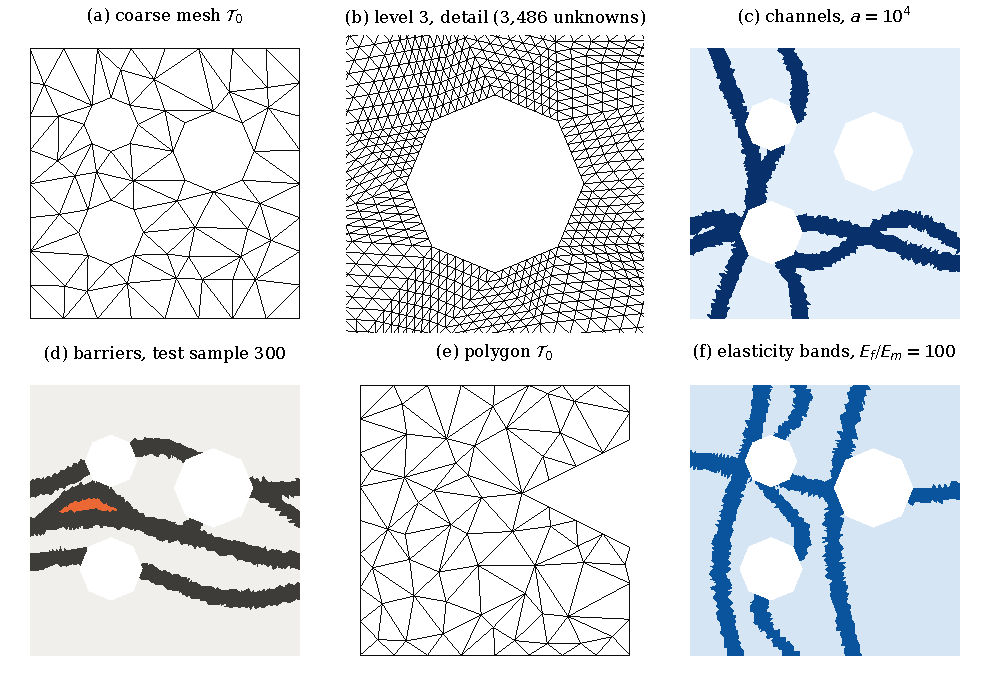
\includegraphics[width=0.92\linewidth]{figures/fig_setup.pdf}
\caption{Meshes and coefficient samples. (a) Unstructured coarse mesh $\mathcal{T}_0$ of the perforated square; (b) detail
of its third uniform refinement; (c) channels, conductive bands $a = 10^4$ (dark) in a unit background; (d) barriers,
insulating bands $a = 10^{-4}$ (dark), with a floating conductive island (orange, geometric label); (e) coarse mesh of the
polygonal domain; (f) elasticity, Young's modulus $100$ times larger in the bands. Field (c) is training sample 0 of held-out
data seed 1; field (d) is test sample 300 of the same seed, chosen as the first test sample whose floating island has more than
30 elements; (f) is training sample 0 of the elasticity data set.}\label{fig:setup}
\end{figure}

\paragraph{Data, training and metrics.} For each experiment 400 coefficient fields are drawn from the random seed $1000+s$,
where $s$ is the \emph{data seed}; samples $0$--$299$ train and $300$--$399$ test. Data seed $0$ was used during development;
all results are on the held-out data seeds $1$--$3$ unless stated otherwise. Each model is trained separately on each data
seed with network initialisation seed $0$; OA-VCB was in addition retrained with initialisation seeds $1$ and $2$
(Section~\ref{sec:initseeds}). All models share the same base loss (the mean of the relative $\ell^2$ and relative energy
errors of the predicted correction), AdamW with a one-cycle schedule (peak learning rate $2\times10^{-3}$), batch size 8 and
300 epochs; models with a Galerkin output add the same loss on their plain cycle output (Section~\ref{sec:output}). Every
learned model in the main comparisons has at most $22{,}000$ parameters (OA-VCB: 20{,}672); an equal cap and schedule do not
make the baselines equally well tuned, and no model was tuned per class. Training used NVIDIA T4 GPUs. The quantity of
interest is the algebraic error with respect to the discrete solution $u$ of $Au=F$, mainly in the energy norm,
$e = \|u - \hat u\|_A/\|u\|_A$; discretisation error is not part of any number. Comparisons are paired per test sample: for a
model and a reference,
\[
  G = \exp\Big(\tfrac1n\textstyle\sum_i \log\big(e^{\mathrm{ref}}_i/e^{\mathrm{model}}_i\big)\Big),\qquad
  W = \tfrac1n\#\{i: e^{\mathrm{model}}_i<e^{\mathrm{ref}}_i\},
\]
so $G>1$ favours the model. The 95\% intervals come from 5{,}000 paired bootstrap resamples of the test samples; they
describe variability over test operators for the trained models at hand, not over training runs. Arithmetic mean errors are
reported alongside; where the two summaries disagree we say so.

\paragraph{Use of generative AI in the research.} The software for this study (data generation, models, training and
evaluation, the classical comparators, the numerical checks of the propositions and the scripts that aggregate the stored
records into tables and figures) was written and run with the assistance of the generative AI system Claude (Anthropic),
under the author's direction; ChatGPT (OpenAI) was used to review the code, the results and the manuscript critically. No
reported number, table or data plot was produced by these tools directly: all are computed by the scripts from the stored
per-sample records (\appref{app:platform}), the principal summaries were recomputed by an independent script from the
per-sample arrays, and the structural properties of Section~\ref{sec:properties} were checked numerically by separate
scripts (\appref{app:impl}). Figure~\ref{fig:schematic} is TikZ source; no figure was created or edited with an image-generating
tool.

\paragraph{Classical comparators.} Next to every learned result we report, on the same samples and from the same $u_c$: the
classical reference of Section~\ref{sec:properties} (one deflated V$(4,4)$ cycle with degree-four Chebyshev smoothers on the
same transfers and Galerkin levels, with Galerkin output); the same cycle without deflation and projection; and two-grid
preconditioned conjugate gradients (weighted Jacobi$(1,1)$ smoothing and an exact level-$(L-1)$ Galerkin coarse solve). For
each test sample we record the first PCG iteration at which the energy error reaches OA-VCB's on that sample. The two
contained classical cycles of Proposition~\ref{prop:containment} are evaluated on the main test sets in \appref{app:impl}
(Table~\ref{tab:contained}): the fixed-interval Chebyshev member is as accurate as the reference to within a few per cent,
and the Jacobi member is $1.35$--$1.82$ times less accurate, so OA-VCB's margin over it is larger ($G = 15$--$16$ on channels,
$2.8$--$3.2$ on barriers).

\paragraph{Learned baselines.}\label{sec:baselines} For context we train learned operators of similar size under the same
protocol (\appref{app:baselines}): \emph{OA-Lift}, our earlier operator-adapted lifting network on the same hierarchy;
\emph{GNN}, a MeshGraphNet-type network; \emph{Transolver}; and Fourier, wavelet, lifting and multigrid neural operators
(FNO, WNO, LiNO, MgNO) on a uniform $63\times63$ grid. The suffix ``-op'' marks variants that receive the information of the
error equation (the scaled residual and, for graph models, the operator weights), like OA-VCB; every baseline starts from
$u_c$ and predicts only the correction. The grid models enter through a mesh--grid bridge whose handicap in the energy norm we
measure (\appref{app:bridge}), so their rows assess our adaptations in this setting, not those architectures on the
uniform-grid problems they were designed for. On the published Darcy benchmark (\appref{app:published}) a faithful FNO port
attains an error comparable to the published value and the official MgNO classes train successfully; these checks of the
implementations and of the benchmark pipeline do not validate every adaptation used in the unstructured-mesh experiments.

\subsection{Accuracy at four update stages}\label{sec:accuracy}\label{sec:channels}\label{sec:barriers}
\begin{table}[tbp]\centering\footnotesize\setlength{\tabcolsep}{4pt}
\caption{Main comparison, held-out data seeds 1--3 (100 test operators each; L3, $k_0=2$). Energy: mean of the three per-seed arithmetic mean relative energy errors. $G$: paired geometric-mean ratio of the classical reference's error to the model's over the pooled 300 samples [95\% CI]; $W$: fraction of samples on which the model is more accurate than the reference. All learned rows have 19{,}521--21{,}603 parameters. The other learned baselines (GNN, and the grid-based FNO-op, WNO-op, LiNO-op, MgNO, MgNO-op, which enter through a mesh--grid bridge) and further classical rows are in Tables~\ref{tab:channels} and~\ref{tab:barriers}.}\label{tab:core}
\begin{adjustbox}{max width=\linewidth}
\begin{tabular}{lllllll}\toprule
 & \multicolumn{3}{c}{channels (contrast $10^4$)} & \multicolumn{3}{c}{barriers (contrast $10^{-4}$)} \\ \cmidrule(lr){2-4}\cmidrule(lr){5-7}
model & energy & $G$ [95\% CI] & $W$ & energy & $G$ [95\% CI] & $W$ \\\midrule
OA-VCB (ours) & 2.75e-3 & 9.89 [9.57, 10.20] & 1.00 & 5.80e-2 & 2.00 [1.86, 2.14] & 0.88 \\
OA-VC (no deflation, plain output) & 3.46e-3 & 8.80 [8.45, 9.12] & 1.00 & 3.73e-1 & 0.61 [0.54, 0.70] & 0.43 \\
OA-Lift & 2.39e-2 & 1.06 [1.04, 1.09] & 0.63 & 3.52e-1 & 0.15 [0.14, 0.16] & 0.00 \\
GNN-op & 3.01e-2 & 0.84 [0.82, 0.86] & 0.19 & 3.61e-1 & 0.12 [0.11, 0.13] & 0.00 \\
Transolver-op & 1.85e-1 & 0.14 [0.13, 0.14] & 0.00 & 3.79e-1 & 0.11 [0.10, 0.12] & 0.00 \\
\midrule
classical reference (Chebyshev, $\nu=4$) & 2.57e-2 & 1 & -- & 8.11e-2 & 1 & -- \\
two-grid PCG, 6 iterations & 2.08e-3 & 14.13 [13.49, 14.81] & 1.00 & 5.05e-2 & 10.36 [8.76, 12.23] & 0.89 \\
$u_c$ alone & 3.73e-1 & 0.07 [0.07, 0.07] & 0.00 & 4.59e-1 & 0.07 [0.07, 0.08] & 0.00 \\
\bottomrule\end{tabular}
\end{adjustbox}
\end{table}

\begin{figure}[tbp]\centering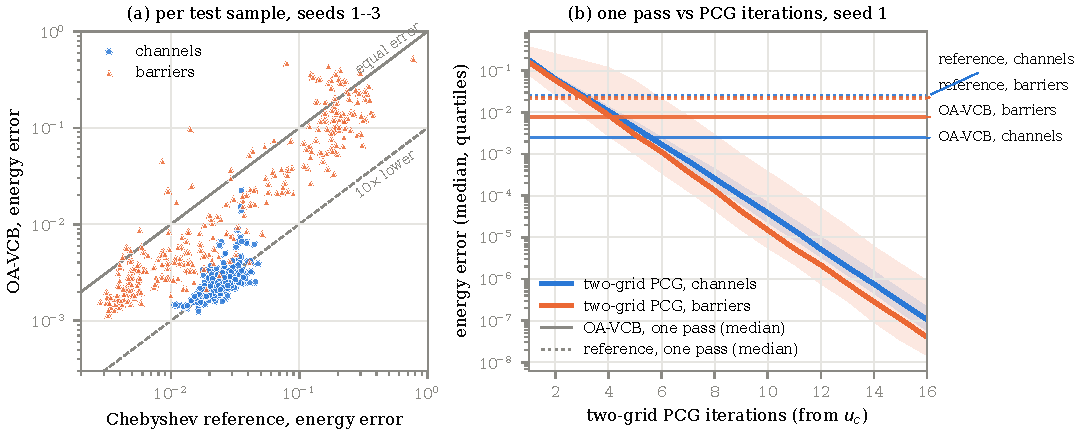
\includegraphics[width=\linewidth]{figures/fig_results.pdf}
\caption{(a) Energy error of OA-VCB against that of the Chebyshev reference on every test sample of held-out seeds 1--3
(300 channel and 300 barrier samples; points below the dashed line are more than ten times more accurate). (b) Energy error
of two-grid PCG from $u_c$ against the number of iterations (median, interquartile band; seed 1), with the median one-pass
errors of OA-VCB (solid) and of the reference (dotted).}\label{fig:results}
\end{figure}
\begin{figure}[tbp]\centering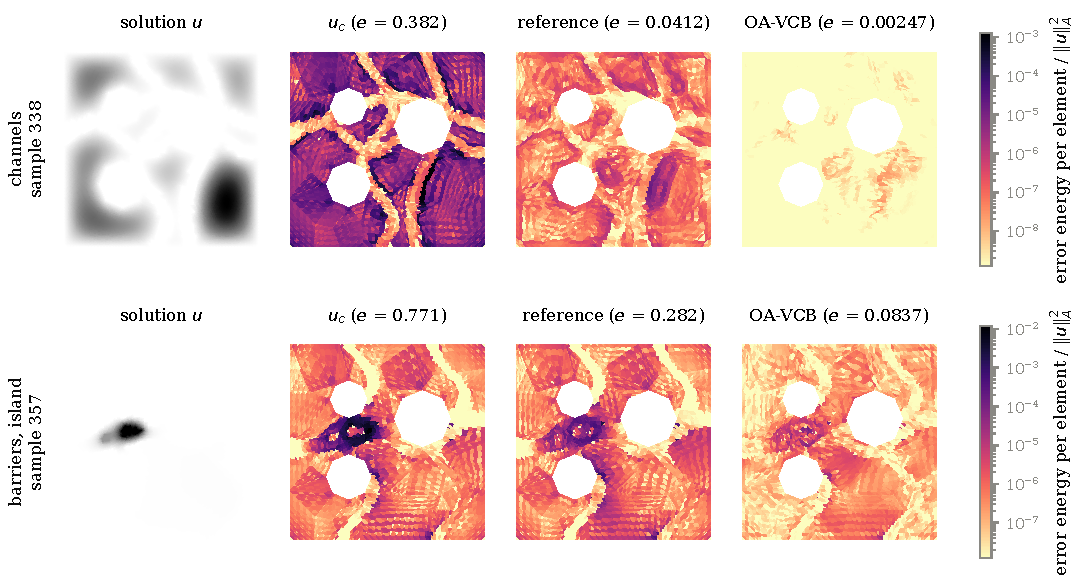
\includegraphics[width=\linewidth]{figures/fig_errormaps.pdf}
\caption{Solution and element-wise energy of the error, $a_e|\nabla(u-\hat u)|^2|T_e|/\|u\|_A^2$, for $\hat u = u_c$, the
Chebyshev reference and OA-VCB, on the median channel test sample (by OA-VCB error) and the median island sample of the
barriers (held-out seed 1). Shared logarithmic colour scale per row.}\label{fig:errormaps}
\end{figure}
\begin{table}[tbp]\centering\footnotesize\setlength{\tabcolsep}{4pt}
\caption{Barriers split by floating islands (geometric label, conductive component touching no Dirichlet node). Mean energy error OA-VCB / classical reference, paired $G$ and $W$ within each group, and OA-VCB's ratio of island to non-island mean error.}\label{tab:islands}
\begin{adjustbox}{max width=\linewidth}
\begin{tabular}{rrlllll}\toprule
seed & islands & with island & $G$, $W$ & without island & $G$, $W$ & ratio \\\midrule
1 & 39 & 0.100 / 0.167 & 1.86, 0.87 & 0.0075 / 0.0165 & 2.33, 0.95 & 13.4 \\
2 & 48 & 0.139 / 0.162 & 1.34, 0.67 & 0.0058 / 0.0140 & 2.70, 0.98 & 24.1 \\
3 & 40 & 0.143 / 0.188 & 1.56, 0.80 & 0.0056 / 0.0135 & 2.23, 0.95 & 25.6 \\
\bottomrule\end{tabular}
\end{adjustbox}
\end{table}

\paragraph{Channels.} OA-VCB is about ten times more accurate than its classical reference in the energy norm
(Table~\ref{tab:core}): $G = 10.23$, $9.76$ and $9.68$ on the three held-out seeds, and more accurate on every one of the 300
test samples (smallest per-sample ratio $1.57$; Figure~\ref{fig:results}(a)). Starting from the same $u_c$, two-grid PCG first
reaches OA-VCB's per-sample energy error after a median of $6$ iterations on each seed (range $5$--$8$;
Figure~\ref{fig:results}(b)). OA-VC, the same learned cycle without deflation and with the plain cycle output, is close
($G = 8.80$); on channels no near-kernel vectors are detected, so the two differ only in the output and its training term.
Among the learned baselines, OA-Lift is $6\%$ more accurate than the reference on average and the others are less accurate
(all nine in \appref{app:baselines}).

\paragraph{Barriers.} Barriers are harder for every method. OA-VCB's margin drops to $G = 2.13$, $1.93$, $1.93$ (pooled
$2.00$), and it is more accurate on $88\%$ of the samples. A minority of samples, those with floating islands, dominates
the mean (Table~\ref{tab:islands}): without islands OA-VCB is $2.2$--$2.7$ times more accurate than the reference, with mean
errors of $5.6$--$7.5\times10^{-3}$, comparable to channels; on island samples its mean error is $13$--$26$ times larger and its
margin shrinks to $G = 1.3$--$1.9$, with losses on $13$--$33\%$ of them. In Figure~\ref{fig:errormaps} the remaining error of
the median island sample is concentrated in and around the island. OA-VCB is never less accurate in energy than $u_c$, as
Proposition~\ref{prop:safeguard} guarantees, whereas OA-VC is less accurate than the reference ($G = 0.61$) and worse than
$u_c$ on $26$ of $300$ samples. Two-grid PCG first reaches OA-VCB's error after a median of $4$--$5$ iterations, with a range of
$2$--$14$ set by the island samples.

\paragraph{Repeated training.}\label{sec:initseeds} OA-VCB was retrained with two further initialisation seeds on every
held-out data set (\appref{app:repeat}, Table~\ref{tab:initseeds}). On channels the nine trained models give
$G = 9.68$--$10.74$, each with $W = 1$; the seed-0 models reported above are the least accurate of the three on every data
seed. On barriers $G = 1.80$--$2.13$ and $W = 0.83$--$0.94$, and the spread over initialisations on one data seed (at most
$0.13$ in $G$) is smaller than the spread over data seeds. These ranges describe training variability on the same test
operators, not independent test observations.

\subsection{The smoothing budget of the comparator}\label{sec:avt}
\begin{table}[tbp]\centering\footnotesize\setlength{\tabcolsep}{4pt}
\caption{Stronger classical smoothers and repeated classical passes, held-out seed 1, measured on one CPU (Intel(R) Xeon(R) Processor @ 2.80GHz, 2 threads; a different machine from Table~\ref{tab:cost}, so OA-VCB was re-timed): energy, the arithmetic mean relative energy error over the 100 test samples (the quantity plotted in Figure~\ref{fig:avt}); $G$, the paired geometric-mean ratio of each classical variant's error to OA-VCB's [95\% CI] (below 1: the classical variant is more accurate in this metric); $W$, the fraction of samples on which OA-VCB is more accurate; and the mean time per sample from $u_c$ with set-up, in ms (classical rows: per-sample minimum over the repetitions; OA-VCB: operator data and batched inference, minimum over the repetitions of the whole-test-set time divided by the number of samples). The eight- and sixteen-step rows exceed the residual-polynomial degree covered by Proposition~\ref{prop:containment} for the four-stage architecture; no learned model with that larger budget was trained.}\label{tab:avt}
\begin{adjustbox}{max width=\linewidth}
\begin{tabular}{lllll}\toprule
method & energy & $G$ [95\% CI] & $W$ & ms \\\midrule
\multicolumn{5}{l}{\emph{channels}: OA-VCB 2.55e-3, 268\,ms} \\
\quad reference, Chebyshev $\nu=4$ (Table~\ref{tab:core}) & 2.59e-2 & 10.23 [9.75, 10.71] & 1.00 & 83 \\
\quad reference, Chebyshev $\nu=8$ & 1.08e-2 & 4.23 [4.00, 4.46] & 1.00 & 79 \\
\quad reference, Chebyshev $\nu=16$ & 4.72e-3 & 1.83 [1.73, 1.93] & 0.99 & 85 \\
\quad reference, symmetric Gauss--Seidel, 4 sweeps & 2.06e-2 & 8.10 [7.69, 8.49] & 1.00 & 77 \\
\quad reference ($\nu=4$) applied twice & 3.50e-3 & 1.30 [1.21, 1.40] & 0.79 & 87 \\
\quad reference ($\nu=4$) applied 3 times & 5.51e-4 & 0.19 [0.17, 0.21] & 0.00 & 88 \\
\multicolumn{5}{l}{\emph{barriers}: OA-VCB 4.36e-2, 273\,ms} \\
\quad reference, Chebyshev $\nu=4$ (Table~\ref{tab:core}) & 7.51e-2 & 2.13 [1.90, 2.38] & 0.92 & 80 \\
\quad reference, Chebyshev $\nu=8$ & 6.47e-2 & 1.25 [1.09, 1.42] & 0.64 & 83 \\
\quad reference, Chebyshev $\nu=16$ & 5.87e-2 & 0.82 [0.69, 0.97] & 0.45 & 85 \\
\quad reference, symmetric Gauss--Seidel, 4 sweeps & 7.30e-2 & 2.11 [1.87, 2.36] & 0.92 & 80 \\
\quad reference ($\nu=4$) applied twice & 2.66e-2 & 0.29 [0.24, 0.35] & 0.13 & 84 \\
\quad reference ($\nu=4$) applied 3 times & 1.21e-2 & 0.05 [0.03, 0.06] & 0.02 & 88 \\
\bottomrule\end{tabular}
\end{adjustbox}
\end{table}

\begin{figure}[tbp]\centering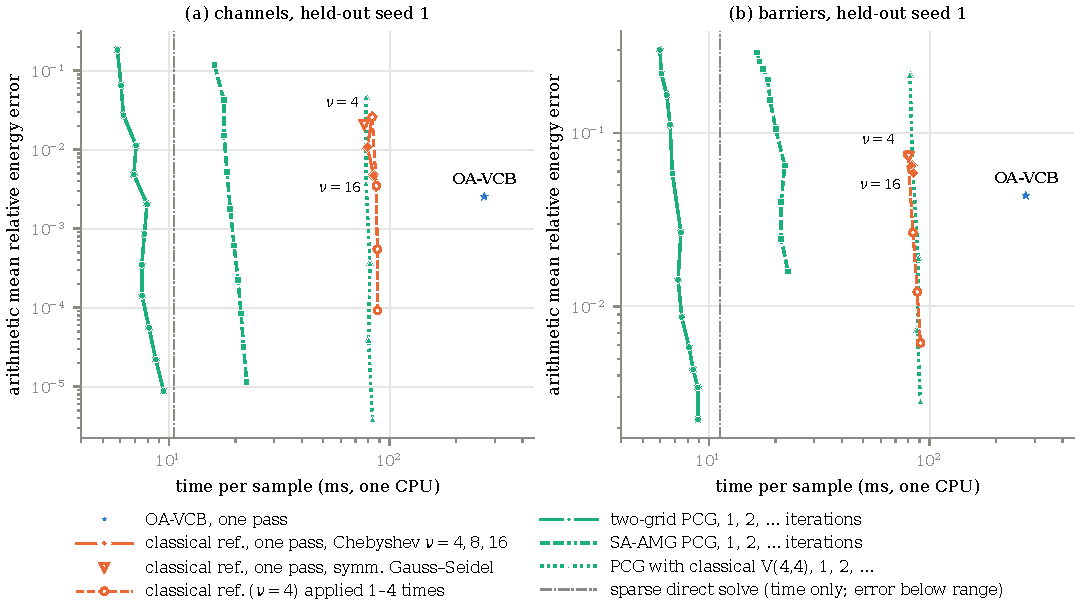
\includegraphics[width=\linewidth]{figures/fig_avt.pdf}
\caption{Arithmetic mean relative energy error against mean time per sample from $u_c$, set-up included, held-out seed 1, all
methods measured in one run on one CPU (Table~\ref{tab:avt}; the paired $G$ of the table is a different summary). Classical
reference: one pass with Chebyshev smoothing of degree $\nu=4$, $8$, $16$ or symmetric Gauss--Seidel, and the $\nu=4$ reference
applied one to four times. PCG curves: one point per iteration. The vertical line marks only the time of the sparse direct
solve, whose error is at solver accuracy, below the plotted range.}\label{fig:avt}
\end{figure}
The margins above compare four learned update stages per pre- and post-smoother with a degree-four Chebyshev reference.
Table~\ref{tab:avt} and Figure~\ref{fig:avt} vary the classical smoothing budget on held-out seed 1, with every method, OA-VCB
included, timed in one run on one machine (\appref{app:platform}). On channels the paired margin falls from $10.2$ at $\nu=4$ to
$4.2$ at $\nu=8$ and $1.8$ at $\nu=16$ ($W = 0.99$). On barriers, sixteen-step Chebyshev reverses the advantage by the paired
geometric-mean metric ($G = 0.82$, with the classical pass more accurate on $55$ of $100$ samples), although OA-VCB retains the
smaller arithmetic mean error ($0.0436$ against $0.0587$). Symmetric Gauss--Seidel with four sweeps is close to the $\nu=4$
reference ($G = 8.1$ and $2.1$). Repeated classical passes give the stronger practical conclusion. Applying the $\nu=4$
reference twice brings it within a paired factor $1.30$ of OA-VCB on channels and makes it $3.5$ times more accurate on barriers
(paired geometric gains; on barriers the mean error is lower as well, $0.0266$); three applications are $5.3$ and $22$ times more
accurate by the paired metric and have lower mean errors on both families ($5.5\times10^{-4}$ and $0.0121$). Because the
operator-adapted hierarchy dominates the classical set-up, every classical variant takes $77$--$88$\,ms per sample, against
$268$--$273$\,ms for OA-VCB on this machine. The eight- and sixteen-step comparisons exceed the residual-polynomial degree
covered by Proposition~\ref{prop:containment} for the four-stage architecture. They test a larger classical smoothing budget; no
learned model with that larger budget was trained. The one-pass margins therefore measure what learning adds at a fixed number
of update stages; at equal cost, on these measurements, the learned pass is not the more accurate one.

\subsection{Cost at matched accuracy}\label{sec:cost}
\begin{table}[tbp]\centering\footnotesize\setlength{\tabcolsep}{4pt}
\caption{Cost per test sample on one CPU (2 threads), channels, held-out seed 1, in ms. Every row starts from the assembled fine matrix; its assembly (1.4 / 5.4 ms, common to all methods) is not included. Per-operator set-up is included in every row; the sparsity patterns of the hierarchy, computed once per mesh (71 / 871 ms), and training are not. Classical rows: mean over the 100 samples of the per-sample minimum over 3 (L3) / 2 (L4) repetitions; OA-VCB operator data and inference: minimum over the repetitions of the whole-test-set time divided by 100. Iteration counts were determined beforehand, untimed, with the reference solution (a matched-accuracy benchmark, not a stopping criterion).}\label{tab:cost}
\begin{adjustbox}{max width=\linewidth}
\begin{tabular}{lll}\toprule
 & L3, $k_0=2$ (3{,}486 unknowns) & L4, $k_0=3$ (14{,}398) \\\midrule
\multicolumn{3}{l}{\emph{OA-VCB (one pass)}} \\
$u_c$ (level-$k_0$ Galerkin factor and solve) & 2.1 & 9.6 \\
operator data (hierarchy, Galerkin levels, $Z$) & 66.6 & 841.3 \\
inference, batch 8 (batch 1) & 96.0 (176.7) & 1{,}561.0 (1{,}461.8) \\
\textbf{total} (batch 8) & 164.8 & 2{,}411.8 \\
\midrule\multicolumn{3}{l}{\emph{single classical pass, error not matched (10 times larger)}} \\
classical reference, from $u_c$ & 60.1 & 769.1 \\
\midrule\multicolumn{3}{l}{\emph{iterative, run to OA-VCB's error on each sample [median; range of iterations]}} \\
two-grid PCG & 5.7 [6; 5--7] & 24.7 [6; 4--8] \\
SA-AMG PCG & 13.5 [5; 4--6] & 41.5 [6; 4--7] \\
PCG with the classical V(4,4) & 61.2 [3; 2--3] & 794.1 [3; 2--3] \\
\midrule\multicolumn{3}{l}{\emph{direct, to solver accuracy}} \\
sparse direct solve (SuperLU) & 8.2 & 48.1 \\
\bottomrule\end{tabular}
\end{adjustbox}
\end{table}

Table~\ref{tab:cost} compares the cost per sample on one CPU of a second machine (\appref{app:platform}). Every row starts
from the assembled fine matrix and includes per-operator set-up; the once-per-mesh sparsity patterns and training are not
included. The iterative methods run, on each sample, exactly the number of iterations that reaches OA-VCB's energy error there;
these counts were determined beforehand with the reference solution, outside the timing, so this is a matched-accuracy
benchmark rather than a deployable stopping rule. Two-grid PCG, SA-AMG PCG and a sparse direct solve are far cheaper than
OA-VCB: at L3, $5.7$, $13.5$ and $8.2$\,ms against $165$\,ms, factors of $29$, $12$ and $20$; at L4 the factors grow to $98$, $58$ and
$50$. The direct solve reaches solver accuracy, much higher than OA-VCB's. From L3 to L4 (4.1 times the unknowns) OA-VCB's time
grows by a factor $15$ and two-grid PCG's by $4.3$. Two components dominate. The operator-adapted hierarchy takes $52$ of the
$67$\,ms of operator data at L3 and $722$ of $841$\,ms at L4; it is a cost of the adapted transfers and their growing operator
complexity, shared with the classical reference, not a cost of learning. The network's CPU inference alone is $17$ (L3) and
$63$ (L4) times the full two-grid PCG time including its set-up, so amortising training over repeated solves cannot make the
learned pass the cheaper route on these configurations. As context only, on the T4 GPU used for training, inference took
$13$\,ms per sample at L3 in batches of eight; optimised implementations, batched GPU operator data and reuse of an operator
for many right-hand sides were not measured.
